\documentclass{gmcmthesis}
\usepackage{pstricks}
\usepackage{tikz}
\usepackage{zhlipsum}
\newcommand{\sol}[1]{
    \colorbox{cyan!50}{[#1]}
}
\usepackage{silence}
\WarningsOff
% 算法环境
\usepackage[linesnumbered,ruled]{algorithm2e}
\renewcommand{\algorithmcfname}{算法}
\AtBeginEnvironment{algorithm}{
    \SetAlgoLined
    \SetKwInOut{Input}{输入}
    \SetKwInOut{Output}{输出}
    \DontPrintSemicolon 
}
\usepackage{csvsimple}
% 设置代码环境
\usepackage{listings}
\lstset{
    basicstyle = \small\ttfamily,           % 基本样式 + 小号字体
    rulesepcolor= \color{gray},             % 代码块边框颜色
    breaklines = true,                  % 代码过长则换行
    numbers = left,                     % 行号在左侧显示
    numberstyle = \small,               % 行号字体
    keywordstyle = \bfseries\color{blue},            % 关键字颜色
    % commentstyle =\color{green!100},        % 注释颜色
    commentstyle=\color{gray!50!black!50},
    stringstyle = \color{red!100},          % 字符串颜色
    frame = shadowbox,                  % 用(带影子效果)方框框住代码块
    showspaces = false,                 % 不显示空格
    columns = fixed,                    % 字间距固定
    %escapeinside={<@}{@>}              % 特殊自定分隔符:<@可以自己加颜色@>
    morekeywords = {as},                % 自加新的关键字(必须前后都是空格)
    deletendkeywords = {eps}        % 删除内定关键字;删除错误标记的关键字用deletekeywords删!
}


\title{中国研究生数学建模竞赛论文标题}
\tenure{二十一} %第x届
\teamid{No.00000001} %参赛队号
\schoolname{国防科技大学}%学校名称
\membera{队员A} %队员A
\memberb{队员B} %队员B
\memberc{队员C} %队员C

\begin{document}
\maketitle
% 目录
% \tableofcontents
% \newpage
% 摘要
\begin{abstract}
    \zhlipsum[1][name = aspirin]

    \keywords{阿司匹林\quad 直肠癌\quad 非甾体抗炎药}
\end{abstract}
% 正文
\section{题目背景}
\subsection{利用zhlipsum随便生成什么内容}
利用 \verb|zhlipsum| 鲁迅的《祝福》。

\zhlipsum[1-20][name = zhufu]

\section{论文正文}
\subsection{插入图片}
本模板不再预先装载任何绘图包(如 \textsf{pstricks,pgf} 等),完全由你自己来决定。

个人觉得 \textsf{pgf} 不错,不依赖于 Postscript。此外还有很多针对 \LaTeX{} 的 GUI 作图工具,如 XFig(jFig), WinFig, Tpx, Ipe, Dia, Inkscape, LaTeXPiX, jPicEdt 等等。本人强烈推荐\textsf{Ipe}。

一般图形都是处在浮动环境中。之所以称为浮动是指最终排版效果图形的位置不一定与源文件中的位置对应,这也是刚使用 \LaTeX{} 同学可能遇到的问题。如果要强制固定浮动图形的位置,请使用 \textsf{float} 宏包,它提供了 \texttt{[H]}(意思是图片就给我放在这里\textcolor{red}{H}ere)参数,但是除非特别需要,不建议使用\texttt{[H]},而是推荐使用\texttt{[htbp]},给\LaTeX{}更多选择。比如图~\ref{fig:ipe}。

\begin{figure}[htbp]
    \centering
    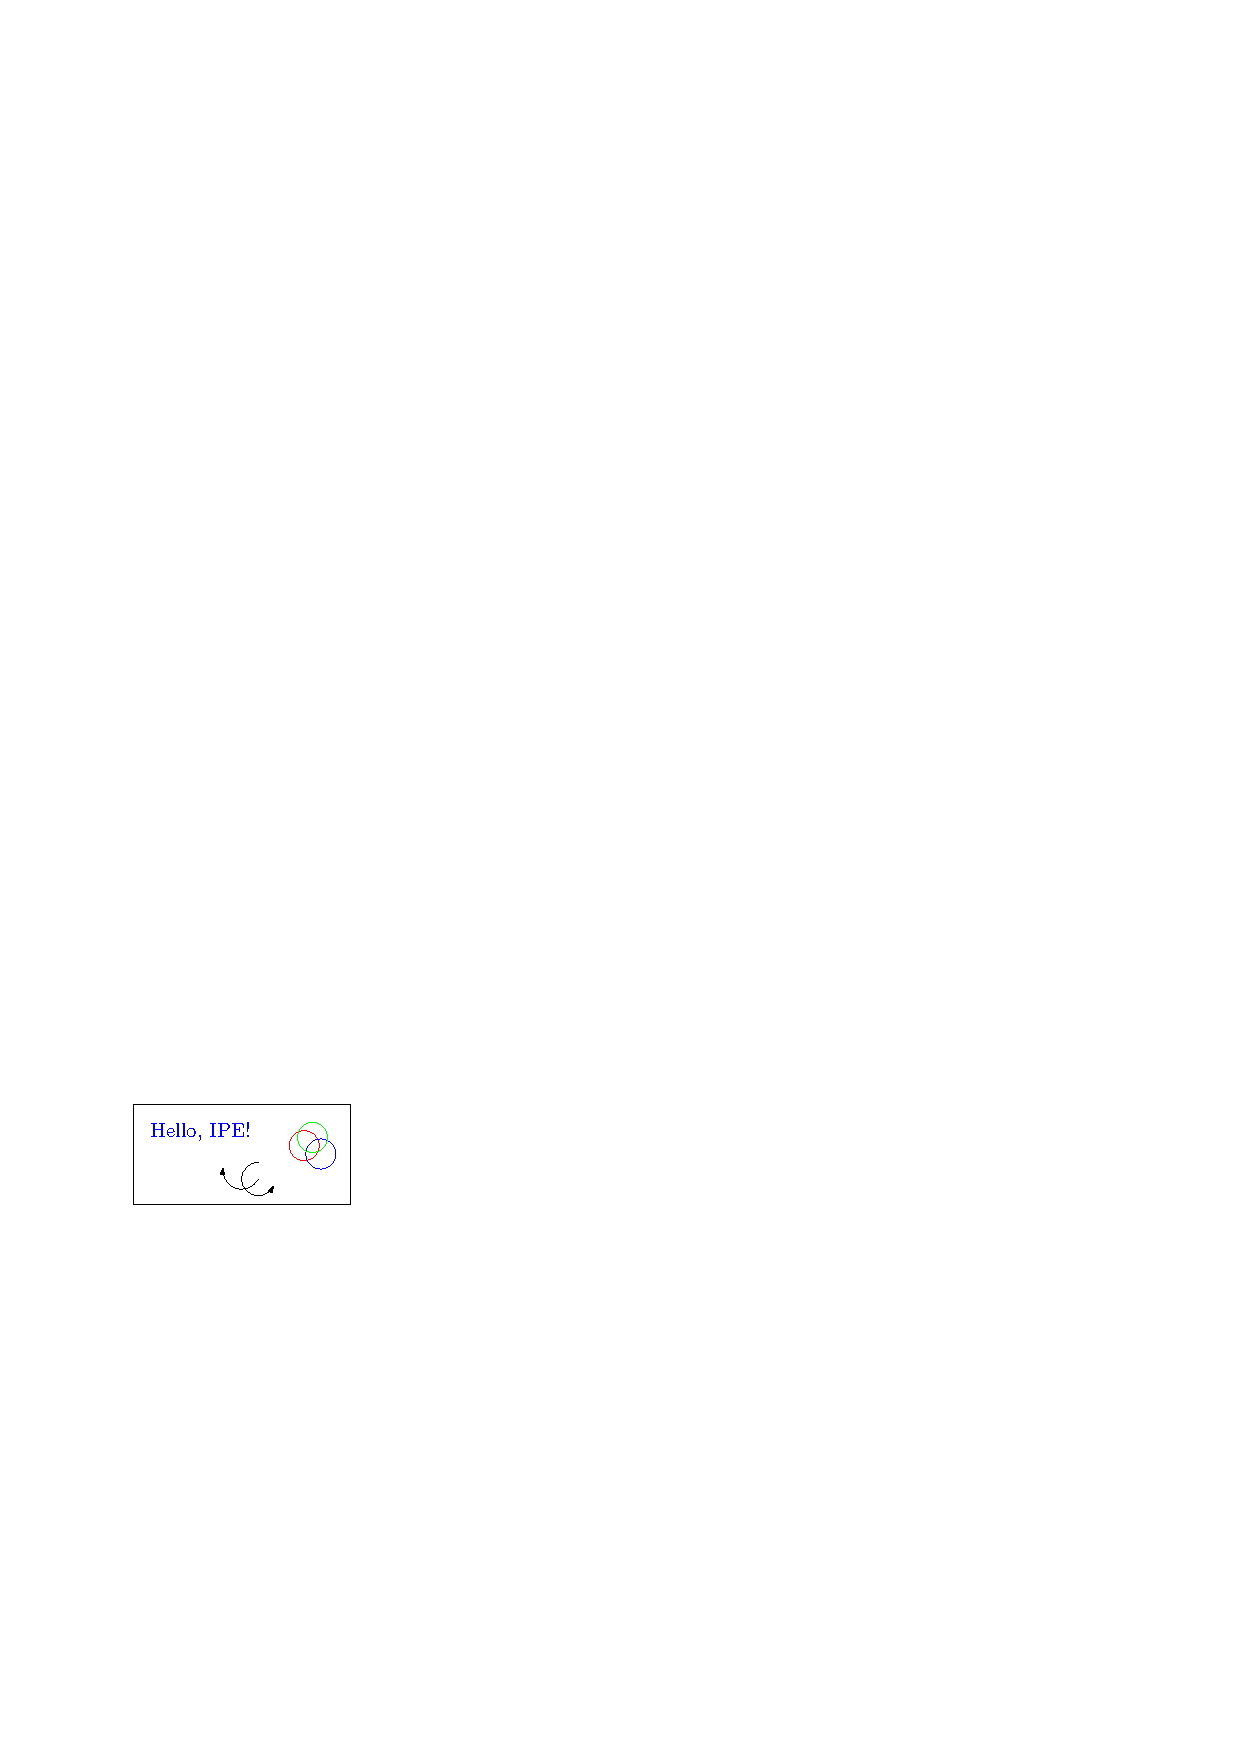
\includegraphics[width=3in]{image/hello.pdf}
    \caption{利用IPE制图}
    \label{fig:ipe}
\end{figure}

若子图共用一个计数器,那么请看图~\ref{fig:big1},它包含两个小图,分别是图~\ref{fig:subfig1}和图~\ref{fig:subfig2}。这里推荐使用\verb|\subfloat|,{\bf 不要再用}\verb|\subfigure|和\verb|\subtable|。
\begin{figure}[htb]
    \centering%
    \subfloat[第一个小图形]{%
      \label{fig:subfig1}
      
\includegraphics[height=2cm]{image/xh.eps}}\hspace{4em}%
    \subfloat[第二个小图形。如果标题很长的话,它会自动换行,这个 caption 就是这样的例子]{%
      \label{fig:subfig2}
      
\includegraphics[height=2cm]{image/xhh.eps}}
    \caption{包含子图形的大图形}
    \label{fig:big1}
\end{figure}

而下面这个例子显示并排$3\times2$的图片,见图~\ref{fig:subfig:3x2}:
\begin{figure}[htb]
    \centering
    \subfloat[]{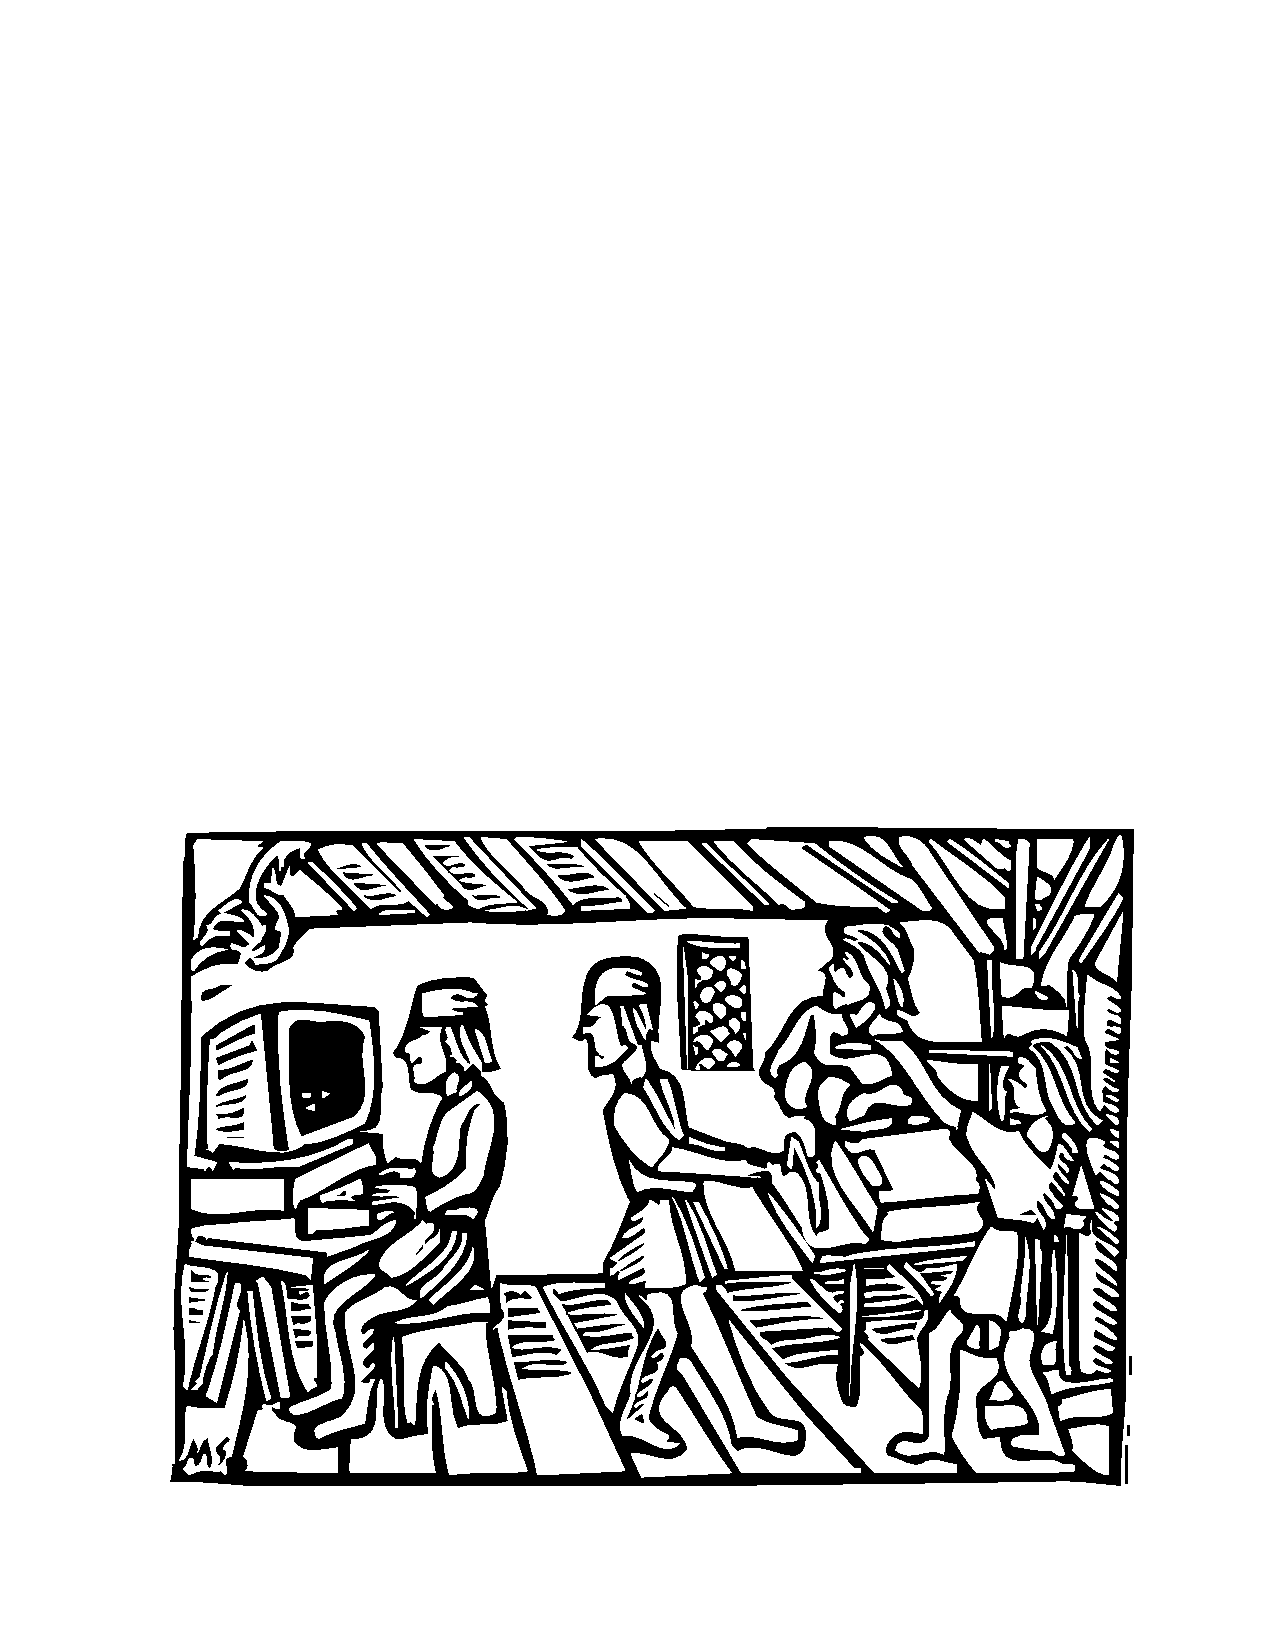
\includegraphics[width=.27\textwidth]{image/typography.pdf}} \qquad
    \subfloat[]{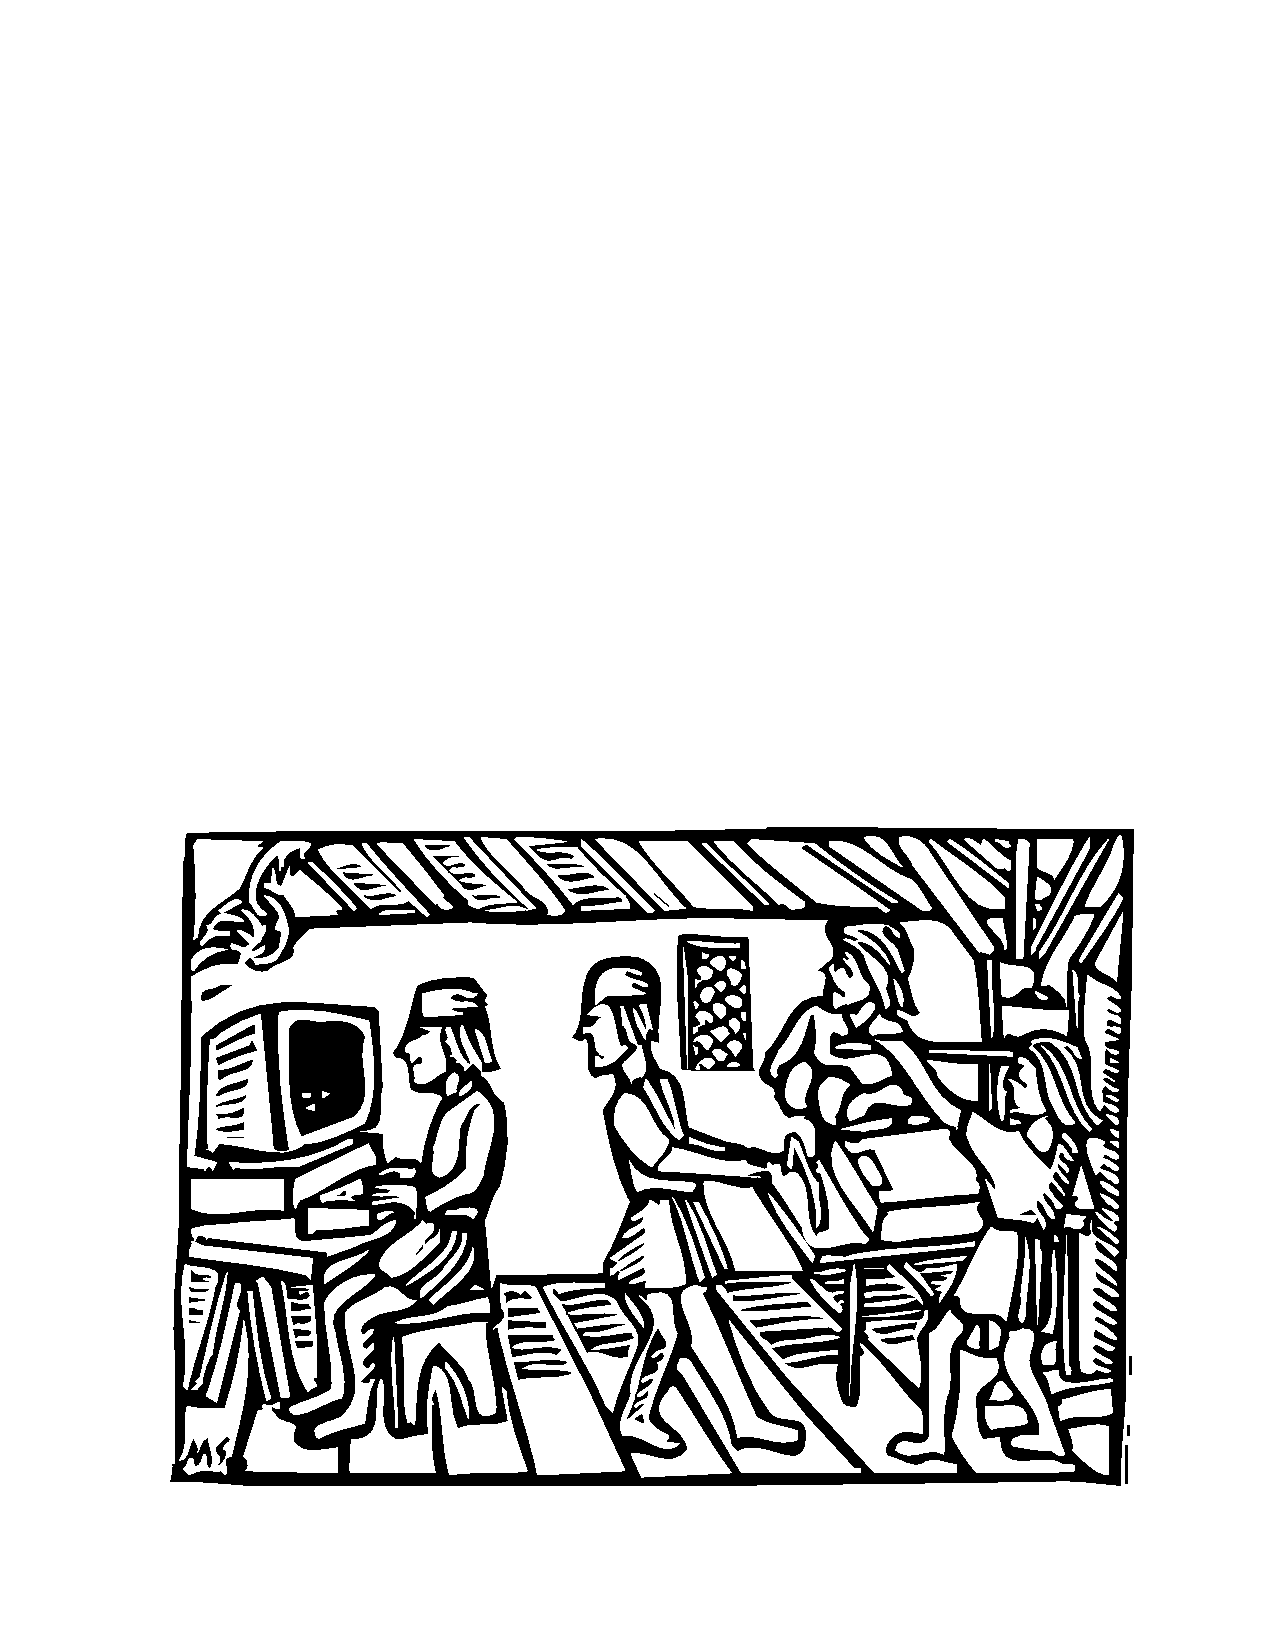
\includegraphics[width=.27\textwidth]{image/typography.pdf}} \qquad
    \subfloat[]{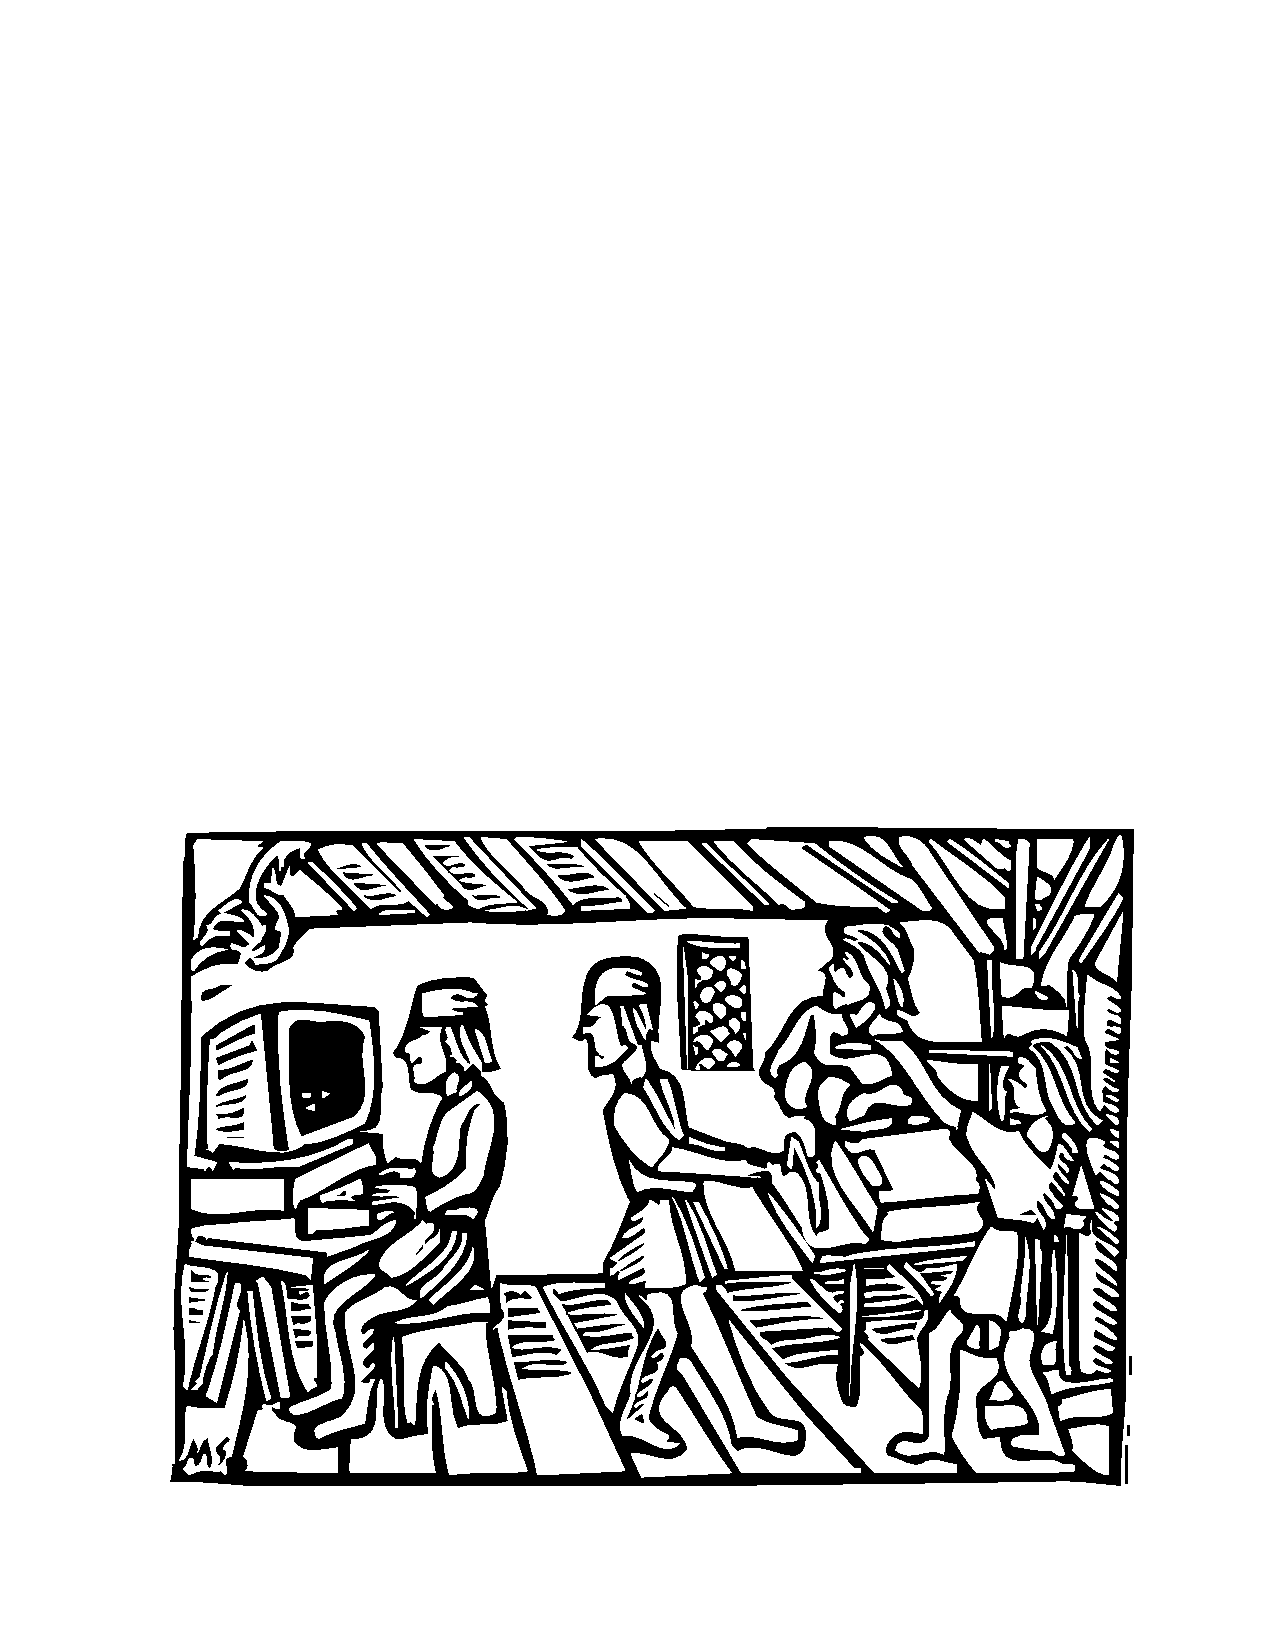
\includegraphics[width=.27\textwidth]{image/typography.pdf}} \qquad
    \subfloat[]{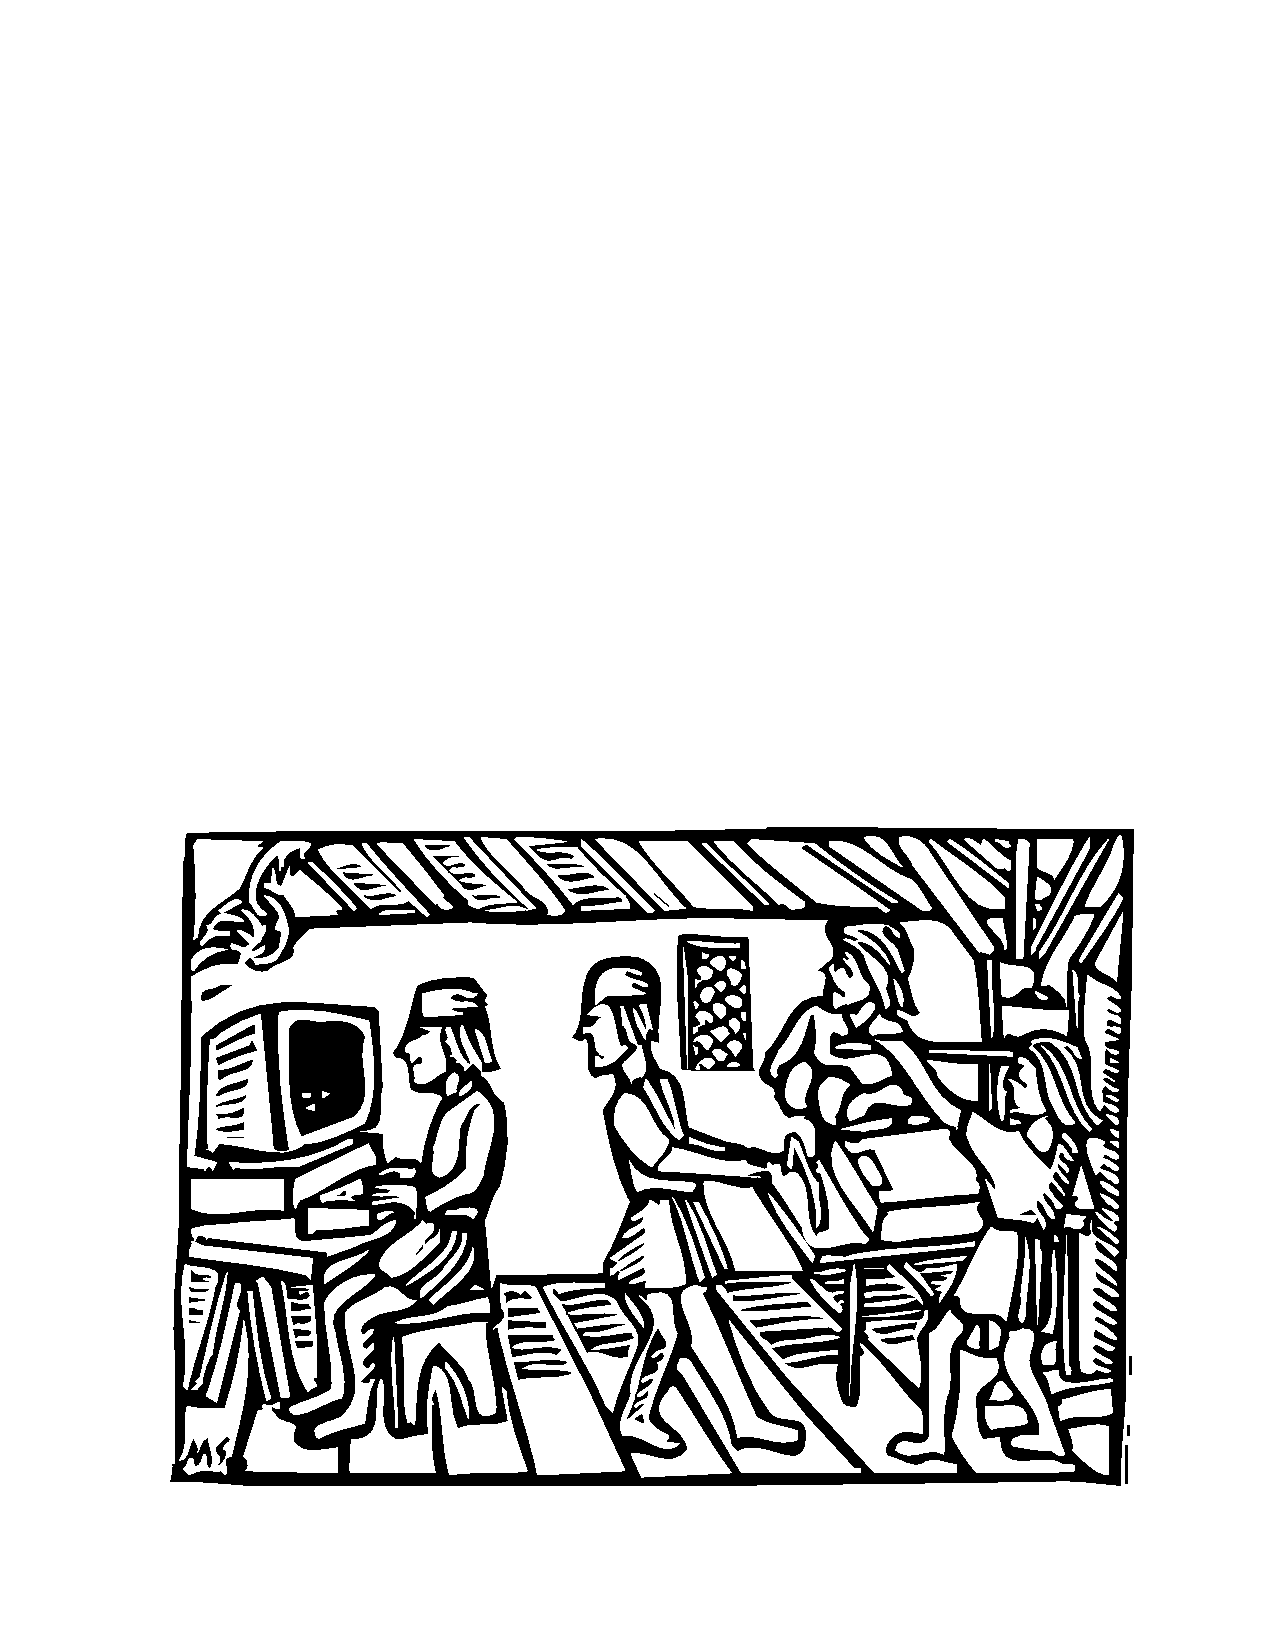
\includegraphics[width=.27\textwidth]{image/typography.pdf}} \qquad
    \subfloat[]{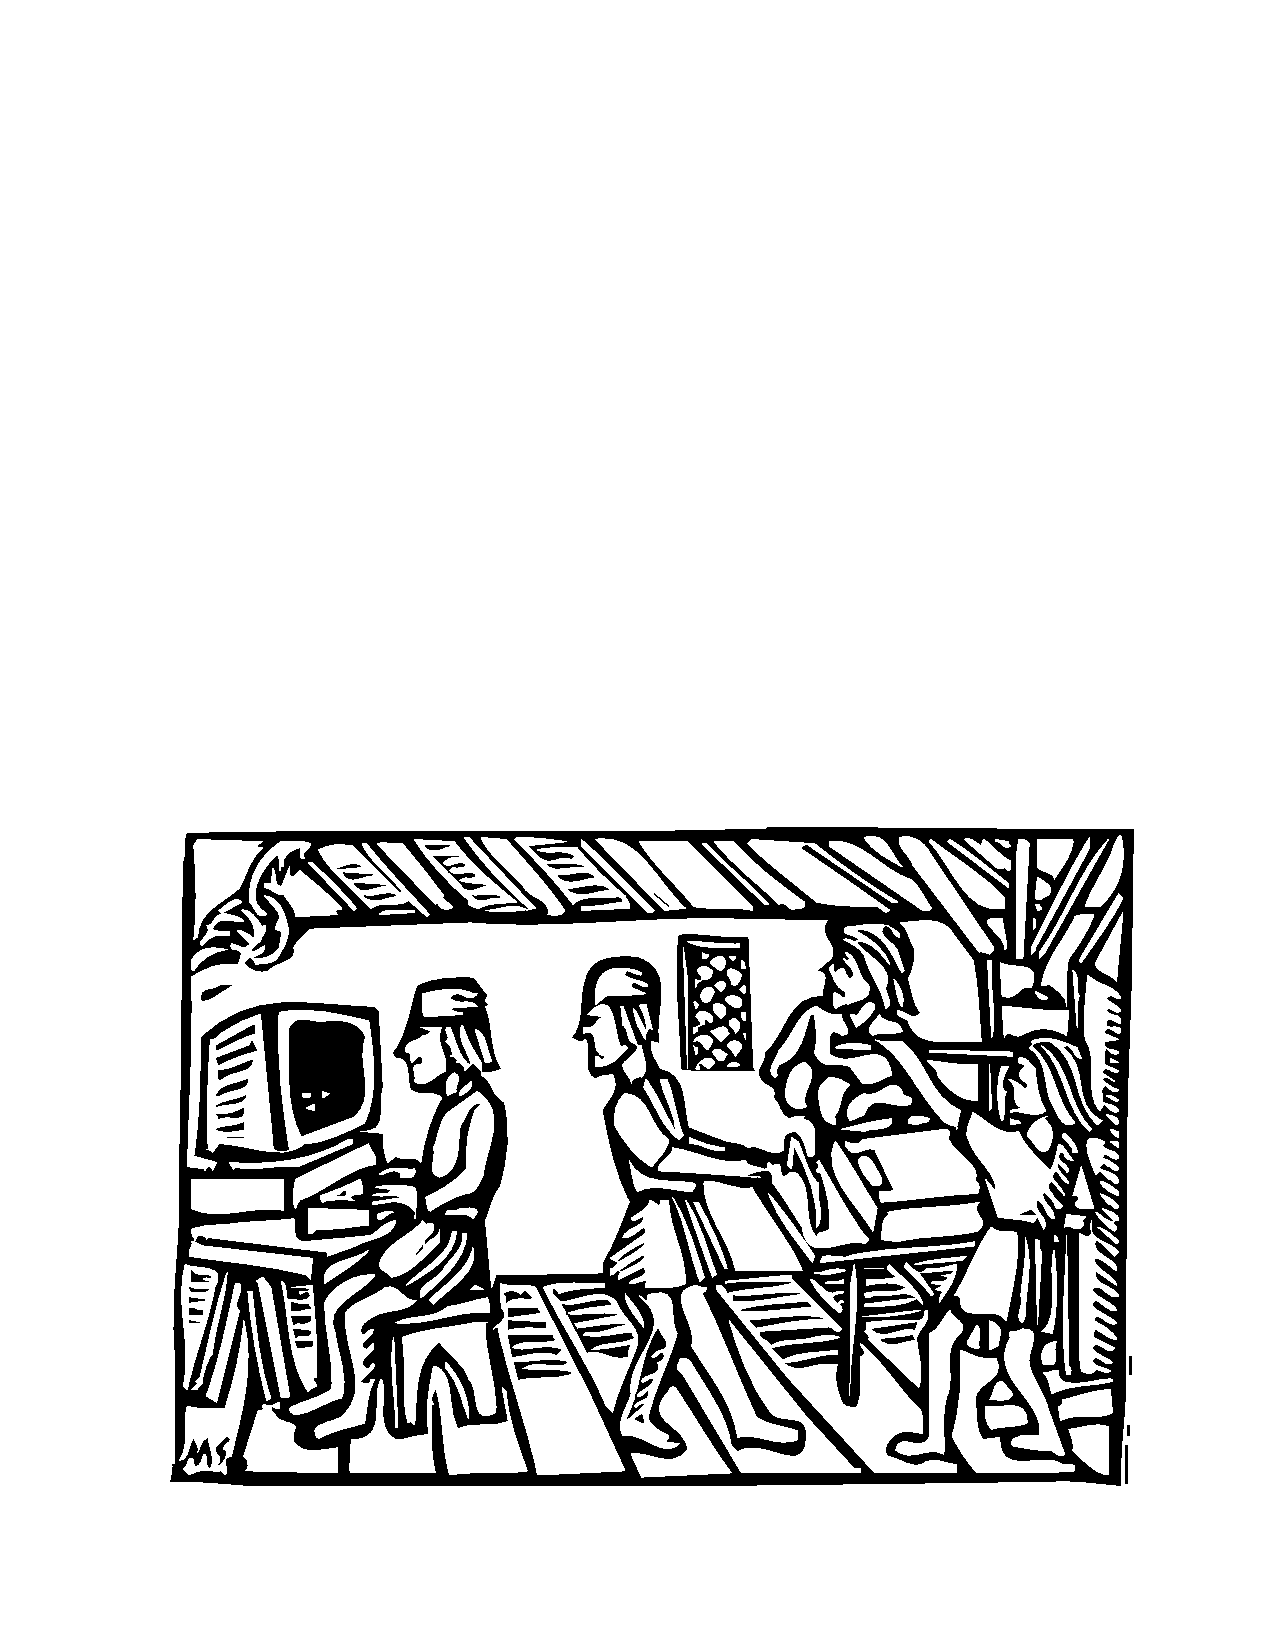
\includegraphics[width=.27\textwidth]{image/typography.pdf}} \qquad
    \subfloat[]{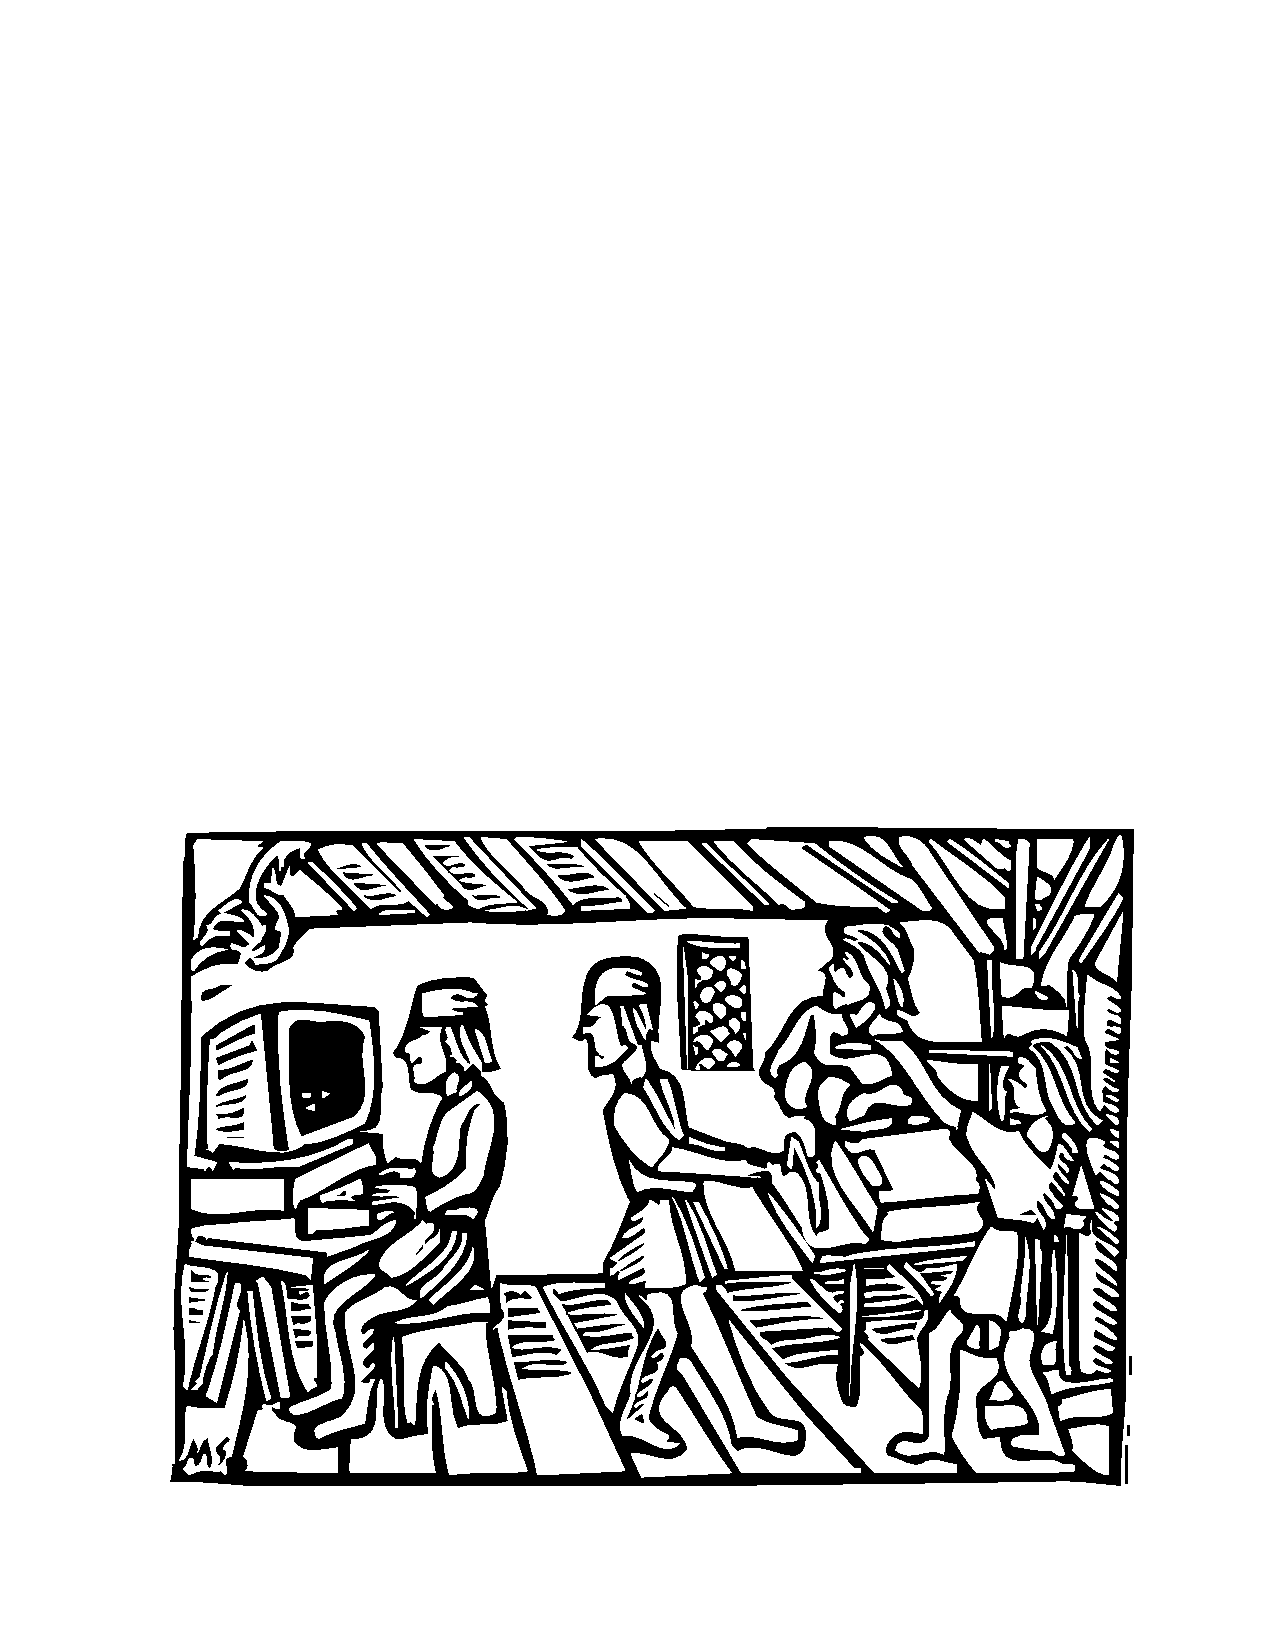
\includegraphics[width=.27\textwidth]{image/typography.pdf}}
    \caption{并排图片}
    \label{fig:subfig:3x2}
\end{figure}

要注意,图~\ref{fig:subfig:3x2}例中\texttt{qquad}相当于\verb|\hspace{2em}|,也就是2个字符的宽度,约0.08倍页宽,图片宽度设定为0.27倍页宽是合适的;在该环境,尽量不要手动换行,所以,不妨自己计算一下!

图形就说这么多,因为大家在写论文是遇到的最大问题不是怎么把图插进去,而是怎样做出专业的、诡异的、震撼的图片来,记得在这时参考前面推荐的那些工具吧,当然必不可少的是Matlab了,至于如何加入中文标注、支持中文等等可以上网去查,但这里{\kai 推荐一点},用好export命令,使得插入图片时尽可能的不要缩放,保证图文的一致性。

\subsection{插入表格}
表格是论文的重要组成部分,我们从简单的表格讲起,到复杂的表格为止。

模板中关于表格的宏包有三个: \textsf{booktabs}、\textsf{array} 和\textsf{longtabular}。三线表建议使用\textsf{booktabs}中提供的,包含toprule、midrule  bottomrule三条命令,简单干脆!它们与\textsf{longtable} 能很好的配合使用。下面来一个表格实例:
\begin{table}[htb]
  \centering
  \begin{minipage}[t]{0.8\linewidth} % 如果想在表格中使用脚注,minipage是个不错的办法
  \caption[模板文件]{模板文件。如果表格的标题很长,那么在表格索引中就会很不美
    观,所以要像 section 那样在前面用中括号写一个简短的标题。这个标题会出现在索
    引中。}
  \label{tab:template-files}
    \begin{tabular*}{\linewidth}{lp{10cm}}
      \toprule[1.5pt]
      {\hei 文件名} & {\hei 描述} \\
      \midrule[1pt]
      gmcmthesis.cls & 模板的文档类\footnote{表格中的脚注} \\
      main.tex & 主文件,编译这个文件\footnote{再来一个}。\\
      preamble.tex & 文章导言区 \\
      \bottomrule[1.5pt]
    \end{tabular*}
  \end{minipage}
\end{table}

表 \ref{tab:template-files} 列举了本模板主要文件及其功能,基本上来说论文中最可能用到的就是这种表格形式了。请大家注意三线表中各条线对应的命令。这个例子还展示了如何在表格中正确使用脚注。如果你不需要在表格中插入脚注,可以将minipage环境去掉。由于\LaTeX{}本身不支持在表格中使用\verb|\footnote|,所以我们不得不将表格放在小页中,而且最好将表格的宽度设置为小页的宽度,这样脚注看起来才更美观。

如果您要排版的表格长度超过一页,那么推荐使用\textsf{longtable}命令。这里随便敲入一些无关的文字,使得正文看上去不是那么的少。表~\ref{tab:performance} 就是 \textsf{longtable} 的简单示例。

\begin{longtable}[c]{c*{6}{r}}
  \caption{实验数据}\label{tab:performance}\\
  \toprule[1.5pt]
    测试程序 & \multicolumn{1}{c}{正常运行} & \multicolumn{1}{c}{同步}
    & \multicolumn{1}{c}{检查点}   & \multicolumn{1}{c}{卷回恢复}
    & \multicolumn{1}{c}{进程迁移} & \multicolumn{1}{c}{检查点} 	\\
    & \multicolumn{1}{c}{时间 (s)} & \multicolumn{1}{c}{时间 (s)}
    & \multicolumn{1}{c}{时间 (s)} & \multicolumn{1}{c}{时间 (s)}
    & \multicolumn{1}{c}{时间 (s)} &  文件(KB)			\\
  \midrule[1pt]%
  \endfirsthead%
  
  \multicolumn{7}{c}{续表~\thetable\hskip1em 实验数据}\\
  
  \toprule[1.5pt]
    测试程序 & \multicolumn{1}{c}{正常运行} & \multicolumn{1}{c}{同步}
    & \multicolumn{1}{c}{检查点}   & \multicolumn{1}{c}{卷回恢复}
    & \multicolumn{1}{c}{进程迁移} & \multicolumn{1}{c}{检查点} 	\\
    & \multicolumn{1}{c}{时间 (s)} & \multicolumn{1}{c}{时间 (s)}
    & \multicolumn{1}{c}{时间 (s)} & \multicolumn{1}{c}{时间 (s)}
    & \multicolumn{1}{c}{时间 (s)} &  文件(KB)			\\
  \midrule[1pt]%
  \endhead%
  \hline%
  
  \multicolumn{7}{r}{续下页}%
  
  \endfoot%
  \endlastfoot%
    CG.A.2 & 23.05   & 0.002 & 0.116 & 0.035 & 0.589 & 32491  \\
    CG.A.4 & 15.06   & 0.003 & 0.067 & 0.021 & 0.351 & 18211  \\
    CG.A.8 & 13.38   & 0.004 & 0.072 & 0.023 & 0.210 & 9890   \\
    CG.B.2 & 867.45  & 0.002 & 0.864 & 0.232 & 3.256 & 228562 \\
    CG.B.4 & 501.61  & 0.003 & 0.438 & 0.136 & 2.075 & 123862 \\
    CG.B.8 & 384.65  & 0.004 & 0.457 & 0.108 & 1.235 & 63777  \\
    MG.A.2 & 112.27  & 0.002 & 0.846 & 0.237 & 3.930 & 236473 \\
    MG.A.4 & 59.84   & 0.003 & 0.442 & 0.128 & 2.070 & 123875 \\
    MG.A.8 & 31.38   & 0.003 & 0.476 & 0.114 & 1.041 & 60627  \\
    MG.B.2 & 526.28  & 0.002 & 0.821 & 0.238 & 4.176 & 236635 \\
    MG.B.4 & 280.11  & 0.003 & 0.432 & 0.130 & 1.706 & 123793 \\
    MG.B.8 & 148.29  & 0.003 & 0.442 & 0.116 & 0.893 & 60600  \\
    LU.A.2 & 2116.54 & 0.002 & 0.110 & 0.030 & 0.532 & 28754  \\
    LU.A.4 & 1102.50 & 0.002 & 0.069 & 0.017 & 0.255 & 14915  \\
    LU.A.8 & 574.47  & 0.003 & 0.067 & 0.016 & 0.192 & 8655   \\
    LU.B.2 & 9712.87 & 0.002 & 0.357 & 0.104 & 1.734 & 101975 \\
    LU.B.4 & 4757.80 & 0.003 & 0.190 & 0.056 & 0.808 & 53522  \\
    LU.B.8 & 2444.05 & 0.004 & 0.222 & 0.057 & 0.548 & 30134  \\
    EP.A.2 & 123.81  & 0.002 & 0.010 & 0.003 & 0.074 & 1834   \\
    EP.A.4 & 61.92   & 0.003 & 0.011 & 0.004 & 0.073 & 1743   \\
    EP.A.8 & 31.06   & 0.004 & 0.017 & 0.005 & 0.073 & 1661   \\
    EP.B.2 & 495.49  & 0.001 & 0.009 & 0.003 & 0.196 & 2011   \\
    EP.B.4 & 247.69  & 0.002 & 0.012 & 0.004 & 0.122 & 1663   \\
    EP.B.8 & 126.74  & 0.003 & 0.017 & 0.005 & 0.083 & 1656   \\
  \bottomrule[1.5pt]
\end{longtable}

\subsection{公式定理}

贝叶斯公式如式~(\ref{eq:bayes}),其中$p(y|\mathbf{x})$为后验;
$p(\mathbf{x})$为先验;分母$p(\mathbf{x})$ 为归一化因子,这是
实际应用中十分恐怖的一个积分式。
\begin{equation}\label{eq:bayes}
  p(y|\mathbf{x}) = \frac{p(\mathbf{x},y)}{p(\mathbf{x})}=
  \frac{p(\mathbf{x}|y)p(y)}{p(\mathbf{x})}
\end{equation}

论文里面公式越多,\TeX{} 就越 happy。再看一个 \textsf{amsmath} 的例子:

\begin{equation}\label{eq:detK2}
  \det\mathbf{K}(t=1,t_1,\dots,t_n)=\sum_{I\in\mathbf{n}}(-1)^{\vert I \vert}
  \prod_{i\in I}t_i\prod_{j\in I}(D_j+\lambda_jt_j)\det\mathbf{A}
  ^{(\lambda)}(\overline{I}|\overline{I})=0.
\end{equation}

当然了,数学中必不可少的是定理:
\begin{theorem}\label{theo:rayleigh solution}
  假定 $X$ 的二阶矩存在:
  \begin{equation}\label{eq:rayleigh solution}
         O_R(\mathbf{x},F)=\sqrt{\frac{\mathbf{u}_1^T\mathbf{A}\mathbf{u}_1} {\mathbf{u}_1^T\mathbf{B}\mathbf{u}_1}}=\sqrt{\lambda_1},
  \end{equation}
  其中 $\mathbf{A}$ 等于 $(\mathbf{x}-EX)(\mathbf{x}-EX)^T$,$\mathbf{B}$ 表示协方差阵 $E(X-EX)(X-EX)^T$,$\lambda_1$ $\mathbf{u}_1$是$\lambda_1$对应的特征向量。
\end{theorem}

下面来看看算法环境的定义和使用。要将\cref{alg:GaussElim}这段顺序Gauss消元法的算法程序改成列主元Gauss消元法,需要在\sol{A} 处添加代码

\begin{algorithm}[H]
  \caption{Gauss列主元消元法}
  \label{alg:GaussElim}
  \Input{$[\boldsymbol{A}\,| \boldsymbol{b}]$}
  \Output{$\boldsymbol{x}$}
  $\boldsymbol{Z} = [\boldsymbol{A}\,| \boldsymbol{b}]$\\
  \For{$k = 1\to n-1$}{
      \tcp*[l]{\colorbox{cyan!50}{A}}
      \For{$i = k+1\to n$}{
          \tcp*[l]{\colorbox{cyan!50}{B}}
          $\boldsymbol{Z}[i,:]\gets \boldsymbol{Z}[i,:]-\dfrac{a_{ik}^{(k)}}{a_{kk}^{(k)}}\boldsymbol{Z}[k,:]$
      }
      \tcp*[l]{\colorbox{cyan!50}{C}}
  }
  $\boldsymbol{A} = \boldsymbol{Z}[:,1:n]$\\
  $\boldsymbol{b} = \boldsymbol{Z}[:,n+1]$\\
  \For{$i = n\to 1$}{
      \tcp*[l]{\colorbox{cyan!50}{D}}
      $\boldsymbol{x}[{i}] = \boldsymbol{b}[i]$\\
      $\boldsymbol{x}[{i}] = \boldsymbol{x}[{i}]-\boldsymbol{A}[i,i+1:]\boldsymbol{x}[i+1:]$\\
      $\boldsymbol{x}[i] = \boldsymbol{x}[i]/\boldsymbol{A}[i,i]$
  }
  \Return {$\boldsymbol{x}$}
\end{algorithm}

\subsection{参考文献}

本模板使用bibtex编译文献数据,文献样式基于gb7714-2015样式针对模板要求要求专门定制。

上标标签的引用命令可使用\textcolor{blue}{\textbf{cite}},行内标签的引用命令可使用\textcolor{blue}{\textbf{upcite}}等。例如:见文献\cite{hutao2024-ji,sobola2001-global,mittelbach2004-latex},就是上标的例子。见文献\upcite{wangfei2017-duo,xiaojie2022-zhi,zhubinglong2020-matlab}就是行内非上标的例子。 

\subsection{其他需知}
作者参加了2023年(第20届)和2024年(第21届)华为杯,这两届的模板的变化只在logo和届次,因此其他使用者在参加不同届的华为杯时可以通过只更改`figure/logo.pdf'和届次\verb|\tenure|快速更改模板。

% 参考文献
\newpage
\bibliographystyle{refs/gmcm}
\bibliography{refs/ref.bib}
% 附录
\newpage
\begin{appendices}
\section{程序代码}
\subsection{python代码}
\lstinputlisting[language = matlab]{code/ADMM.m}
\section{使用csvsimple宏包生成\LaTeX{}表格}
\subsection{结果}
使用csvsimple 宏包的最简单方式是直接\verb|\csvautotabular|命令生成表格,其代码如下,生成的表格如\cref{tab:csvautotabular}所示。
\begin{table}[htbp]
    \centering
    \caption{使用 csvautotabular 命令生成表格\label{tab:csvautotabular}}
    \csvautotabular{table/name-gender-age.csv}
\end{table}
\subsection{logo}
最后自己用\textsf{Ipe}制作了本文档的logo。
\begin{figure}[htbp]
    \centering
    
\includegraphics[width = 2.5in]{image/gmcmthesis.pdf}
    \caption{用\textsf{Ipe}制作的logo}
\end{figure}
\subsection{较长的标题}
% Table generated by Excel2LaTeX from sheet '数据'
\begin{table}[htbp]
    \centering
    \caption{第1、2、4 问的详细定位结果, 每一问的物体数量皆为2个, 给出了物体的直角坐标、物体极坐标、物体的反射系数, 以及利用重建的位置数据生成观测信号与原始观测信号间的$\ell_2$范数误差.}
    \resizebox{\textwidth}{!}{
    \begin{tabular}{ccccc}
        \toprule[1.5pt]
        \multicolumn{1}{c}{数据集} & 物体直角坐标$(x, y)$ & 物体极坐标$(r, \theta)$ & 物体反射系数 & 观测信号的重建误差 \\
        \midrule[1pt]
        \multicolumn{1}{c}{\multirow{2}[2]{*}{1, 无噪声数据}} &   (-0.0183, 7.0048) & (7.0048, -0.0026) & 3.9952 + 3.0058i                  & \multirow{2}[2]{*}{0.0454} \\
            & (0.0184, 7.0048) & (7.0048, 0.0026) & -2.9940 - 4.0046i &  \\
        \hline
        \multicolumn{1}{c}{\multirow{2}[2]{*}{2, 含噪声数据}} &   (-0.0447, 8.2056) & (8.2057, -0.0054) & 4.3719 + 2.0751i               & \multirow{2}[2]{*}{209.4977} \\
            & (0.0447, 8.2056) & (8.2058, 0.0054) & -3.8427 - 2.9398i &  \\
        \hline
        \multicolumn{1}{c}{\multirow{2}[2]{*}{4, 天线老化数据}} &    (0.0159, 6.1042) & (6.1042, 0.0026) & -2.5414 - 4.2246i           & \multirow{2}[2]{*}{169.0732} \\
            & (-0.0158, 6.0041) & (6.0041, -0.0026) & 3.8456 + 3.0986i &  \\
        \bottomrule[1.5pt]
    \end{tabular}%
    }
    \label{tab:data}%
\end{table}%
\end{appendices}
\end{document}
